\begin{table}[htbp]
\centering
\resizebox{\textwidth}{!}{%
\begin{tabular}{lccc}
\hline
Cut & Bkg Events & Signal Events & Sig/Bkg Ratio \\
\hline
Before cuts & 1950.26 $\pm$ 6.61 & 3.12 & 0.00 \\
Max $\cos(\theta_{\mathrm{beam}})$ & 106.34 $\pm$ 1.54 & 1.43 & 0.01 \\
Tail Length Density & 23.09 $\pm$ 0.72 & 0.94 & 0.04 \\
Cut on $C_{140-150}$ & 6.65 $\pm$ 0.39 & 0.63 & 0.09 \\
ROI Z close to vertex & 1.79 $\pm$ 0.20 & 0.54 & 0.30 \\
N daughter particles & 0.81 $\pm$ 0.13 & 0.47 & 0.59 \\
Vertex fiducial volume & 0.65 $\pm$ 0.12 & 0.46 & 0.71 \\
Cut on $C_{40-50}$ & 0.56 $\pm$ 0.11 & 0.44 & 0.78 \\
ROI Z size & 0.49 $\pm$ 0.10 & 0.44 & 0.88 \\
Cut on $C_{0-10}$ & 0.45 $\pm$ 0.10 & 0.41 & 0.92 \\
\hline
Surviving events & 0.02\% & 13.1\% & \\
\hline
\end{tabular}
}
\caption{Expected number of events during all steps of the selection, weighted to one hour of beam-on data.}
\label{tab:filter_evolution}
\end{table}



\begin{figure}[!h]
    \centering
    
\includegraphics[width=0.32\linewidth]{sections/appendix/w133_nocut_normalized/sig_bkg_max_directionZ_directionZ2_spectrum_normalized.png}
    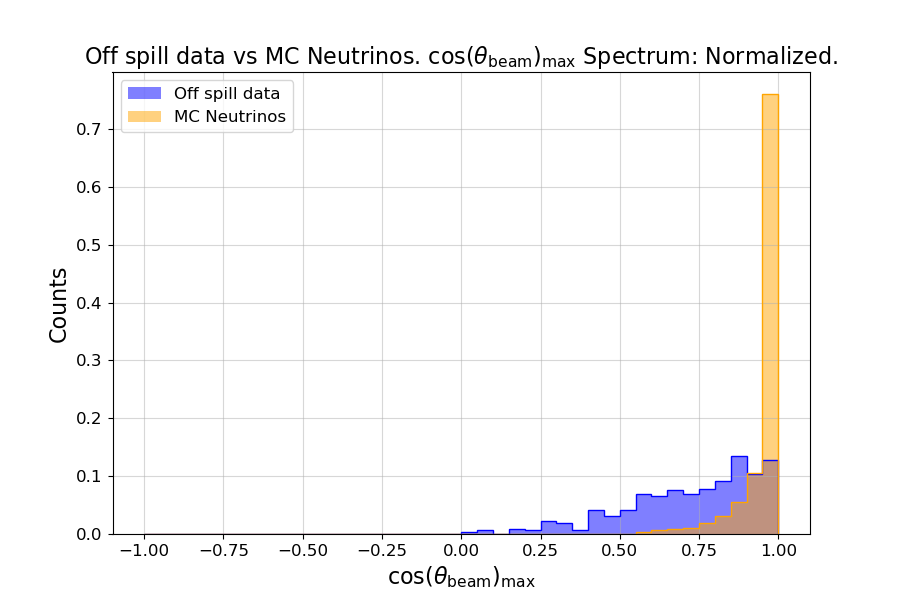
\includegraphics[width=0.32\linewidth]{sections/appendix/w133_yescut_normalized/sig_bkg_max_directionZ_directionZ2_spectrum_normalized.png}
    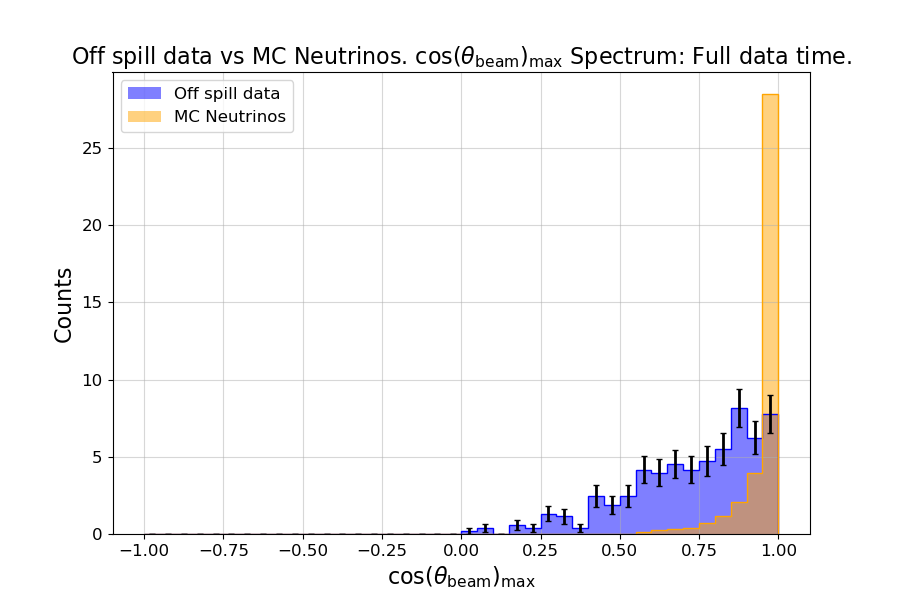
\includegraphics[width=0.32\linewidth]{sections/appendix/w133_yescut_fulltime/sig_bkg_max_directionZ_directionZ2_spectrum_full_sig_time.png}
    \caption{Left: $\cos(\theta_{\mathrm{beam}})_{\text{max}}$ distribution before cuts, area normalized to 1. Middle: $\cos(\theta_{\mathrm{beam}})_{\text{max}}$ distribution with all other cuts applied, area normalized to 1. Right: $\cos(\theta_{\mathrm{beam}})_{\text{max}}$ distribution with all other cuts applied, normalized to the expected number of events in the available data.}
    \label{fig:maxZ}
\end{figure}

\begin{figure}[!h]
    \centering
    
\includegraphics[width=0.32\linewidth]{sections/appendix/w133_nocut_normalized/sig_bkg_tail_density_normalized.png}
    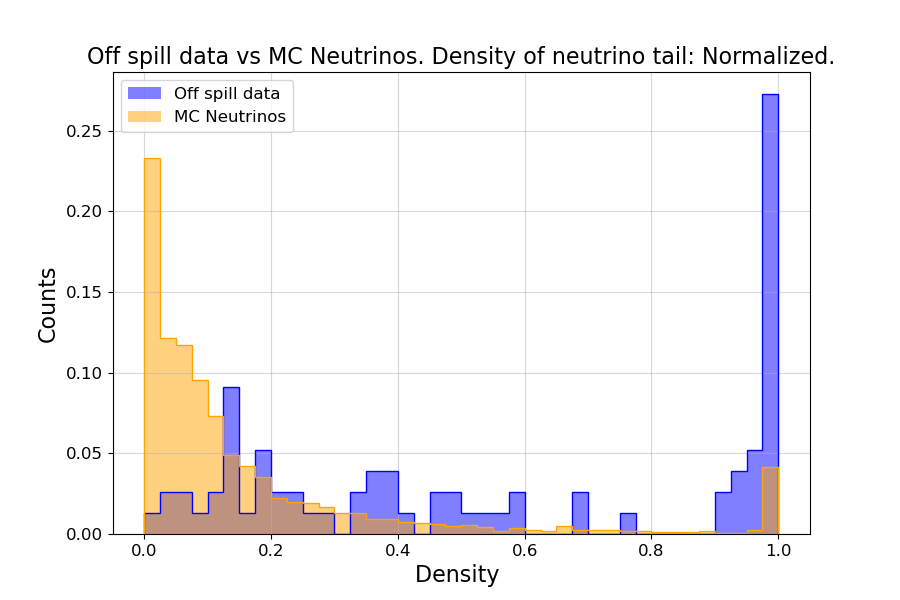
\includegraphics[width=0.32\linewidth]{sections/appendix/w133_yescut_normalized/sig_bkg_tail_density_normalized.png}
    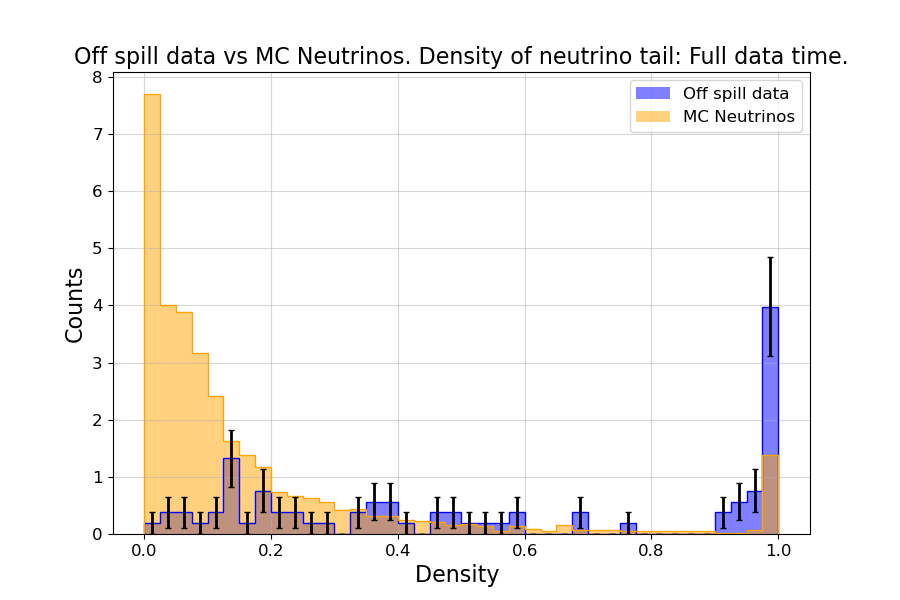
\includegraphics[width=0.32\linewidth]{sections/appendix/w133_yescut_fulltime/sig_bkg_tail_density_full_sig_time.png}
    \caption{Left: Tail length density distribution before cuts, area normalized to 1. Middle: Tail length density distribution with all other cuts applied, area normalized to 1. Right: Tail length density distribution with all other cuts applied, normalized to the expected number of events in the available data.}
    \label{fig:tailDensity}
\end{figure}


\begin{figure}[!h]
    \centering
    
\includegraphics[width=0.32\linewidth]{sections/appendix/w133_nocut_normalized/sig_bkg_energyDepositedInFifteenth10cm_spectrum_normalized.png}
    
\includegraphics[width=0.32\linewidth]{sections/appendix/w133_yescut_normalized/sig_bkg_energyDepositedInFifteenth10cm_spectrum_normalized.png}
    
\includegraphics[width=0.32\linewidth]{sections/appendix/w133_yescut_fulltime/sig_bkg_energyDepositedInFifteenth10cm_spectrum_full_sig_time.png}
    \caption{Left: Charge in range 140-150 cm from the vertex before cuts, area normalized to 1. Middle: Charge in range 140-150 cm from the vertex with all other cuts applied, area normalized to 1. Right: Charge in range 140-150 cm from the vertex with all other cuts applied, normalized to the expected number of events in the available data.}
    \label{fig:energyFifteenth10}
\end{figure}

\begin{figure}[!h]
    \centering
    
\includegraphics[width=0.32\linewidth]{sections/appendix/w133_nocut_normalized/sig_bkg_energyDepositedInFifth10cm_spectrum_normalized.png}
    
\includegraphics[width=0.32\linewidth]{sections/appendix/w133_yescut_normalized/sig_bkg_energyDepositedInFifth10cm_spectrum_normalized.png}
    
\includegraphics[width=0.32\linewidth]{sections/appendix/w133_yescut_fulltime/sig_bkg_energyDepositedInFifth10cm_spectrum_full_sig_time.png}
    \caption{Left: Charge in range 40-50 cm from the vertex before cuts, area normalized to 1. Middle: Charge in range 40-50 cm from the vertex with all other cuts applied, area normalized to 1. Right: Charge in range 40-50 cm from the vertex with all other cuts applied, normalized to the expected number of events in the available data.}
    \label{fig:energyFifth10}
\end{figure}

\begin{figure}[!h]
    \centering
    
\includegraphics[width=0.32\linewidth]{sections/appendix/w133_nocut_normalized/sig_bkg_energyDepositedInFirst10cm_spectrum_normalized.png}
    
\includegraphics[width=0.32\linewidth]{sections/appendix/w133_yescut_normalized/sig_bkg_energyDepositedInFirst10cm_spectrum_normalized.png}
    
\includegraphics[width=0.32\linewidth]{sections/appendix/w133_yescut_fulltime/sig_bkg_energyDepositedInFirst10cm_spectrum_full_sig_time.png}
    \caption{Left: Charge in range 0-10 cm from the vertex before cuts, area normalized to 1. Middle: Charge in range 0-10 cm from the vertex with all other cuts applied, area normalized to 1. Right: Charge in range 0-10 cm from the vertex with all other cuts applied, normalized to the expected number of events in the available data.}
    \label{fig:energyFirst10}
\end{figure}



\begin{figure}[!h]
    \centering
    
\includegraphics[width=0.32\linewidth]{sections/appendix/w133_nocut_normalized/sig_bkg_distance_vertexZ_to_ROI_start_normalized.png}
    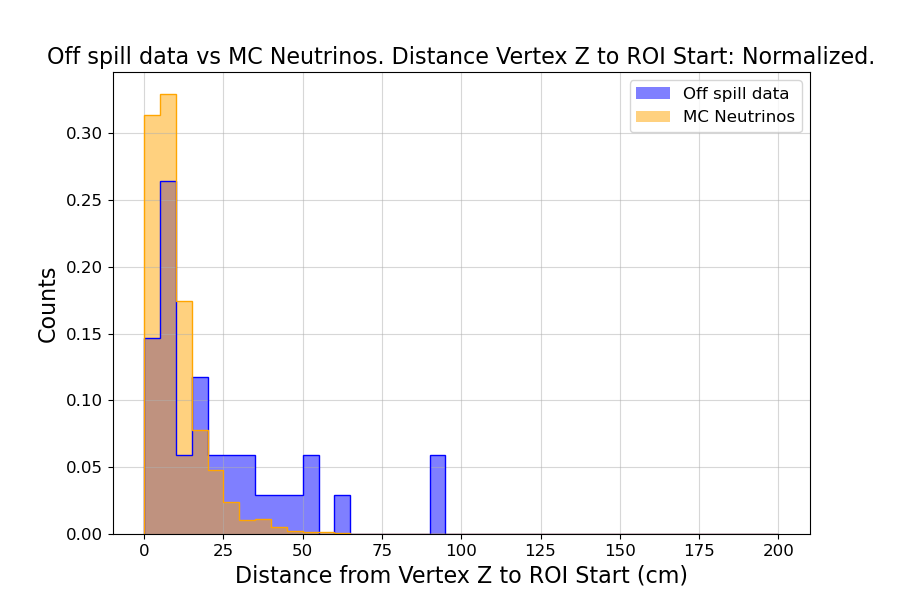
\includegraphics[width=0.32\linewidth]{sections/appendix/w133_yescut_normalized/sig_bkg_distance_vertexZ_to_ROI_start_normalized.png}
    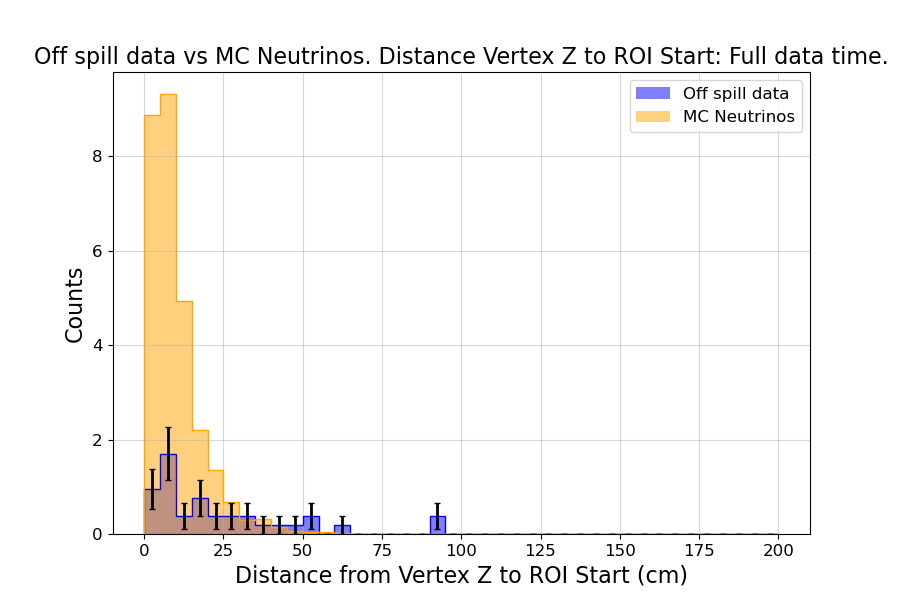
\includegraphics[width=0.32\linewidth]{sections/appendix/w133_yescut_fulltime/sig_bkg_distance_vertexZ_to_ROI_start_full_sig_time.png}
    \caption{Left: Distribution of the distance between the vertex Z and the start of the ROI before cuts, area normalized to 1. Middle: Distribution of the distance between the vertex Z and the start of the ROI with all other cuts applied, area normalized to 1. Right: Distribution of the distance between the vertex Z and the start of the ROI with all other cuts applied, normalized to the expected number of events in the available data.}
    \label{fig:ROIdistance}
\end{figure}

\begin{figure}[!h]
    \centering
    
\includegraphics[width=0.32\linewidth]{sections/appendix/w133_nocut_normalized/sig_bkg_numberOfPFParticles_spectrum_normalized.png}
    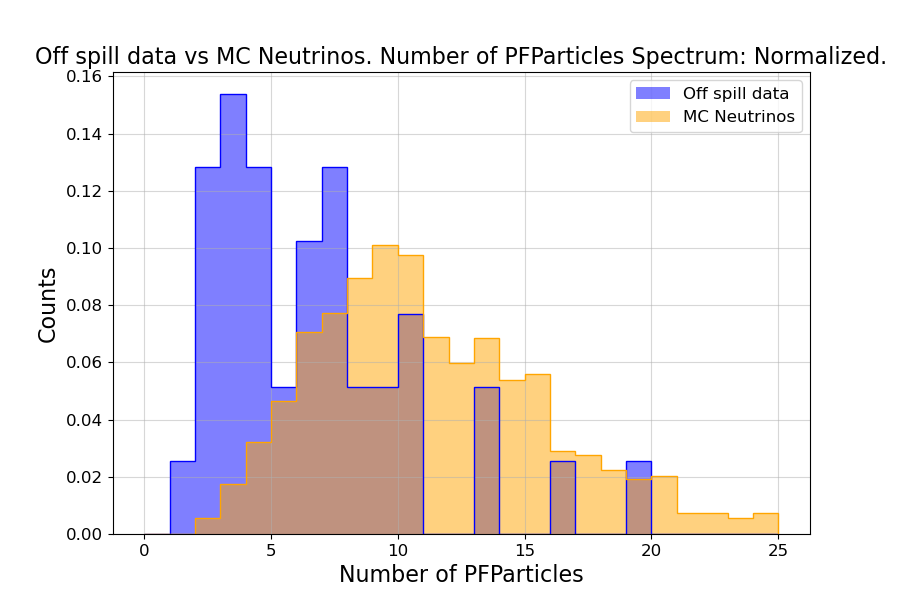
\includegraphics[width=0.32\linewidth]{sections/appendix/w133_yescut_normalized/sig_bkg_numberOfPFParticles_spectrum_normalized.png}
    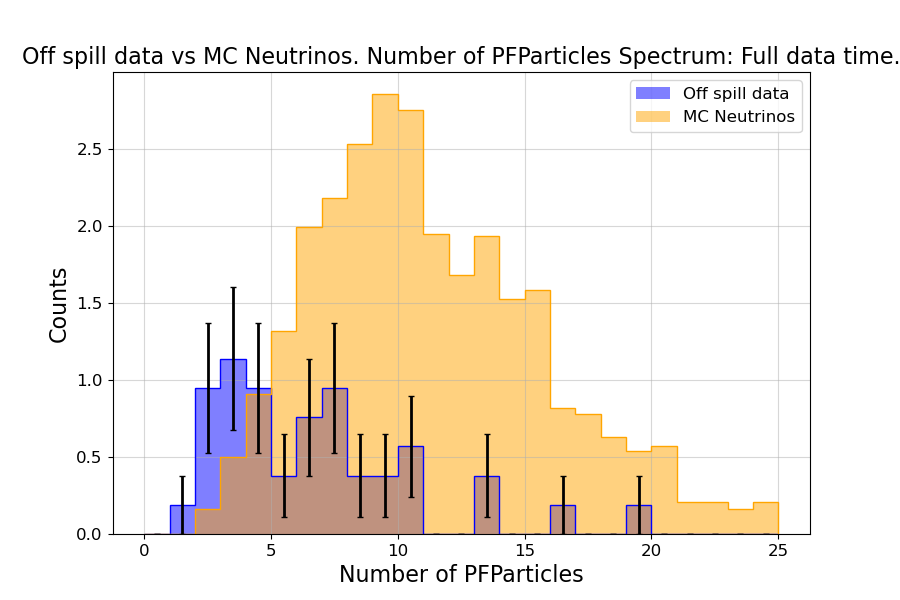
\includegraphics[width=0.32\linewidth]{sections/appendix/w133_yescut_fulltime/sig_bkg_numberOfPFParticles_spectrum_full_sig_time.png}
    \caption{Left: Number of daughter particles before cuts, area normalized to 1. Middle: Number of daughter particles with all other cuts applied, area normalized to 1. Right: Number of daughter particles with all other cuts applied, normalized to the expected number of events in the available data.}
    \label{fig:nPFPs}
\end{figure}



\begin{figure}[!h]
    \centering
    
\includegraphics[width=0.32\linewidth]{sections/appendix/w133_nocut_normalized/sig_bkg_vertexZ_spectrum_normalized.png}
    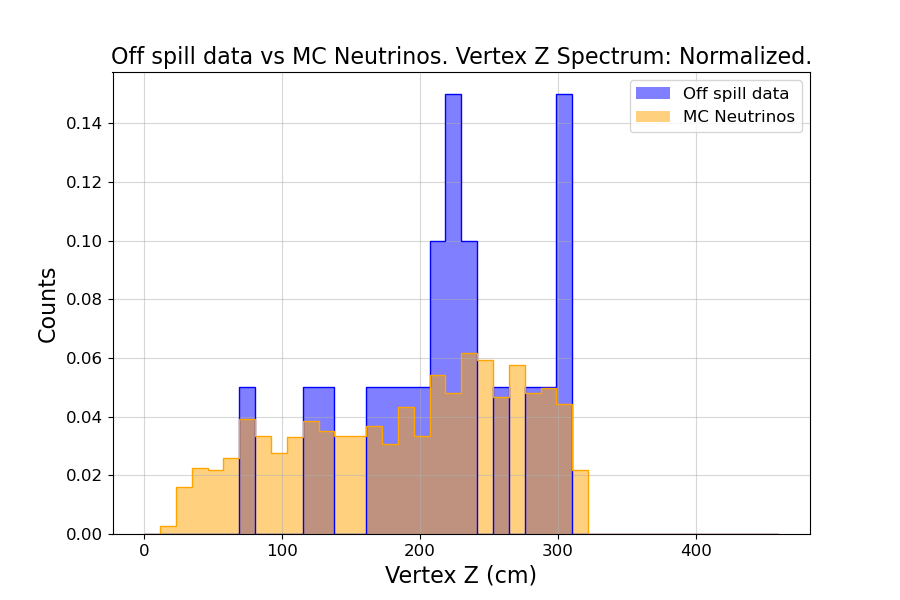
\includegraphics[width=0.32\linewidth]{sections/appendix/w133_yescut_normalized/sig_bkg_vertexZ_spectrum_normalized.png}
    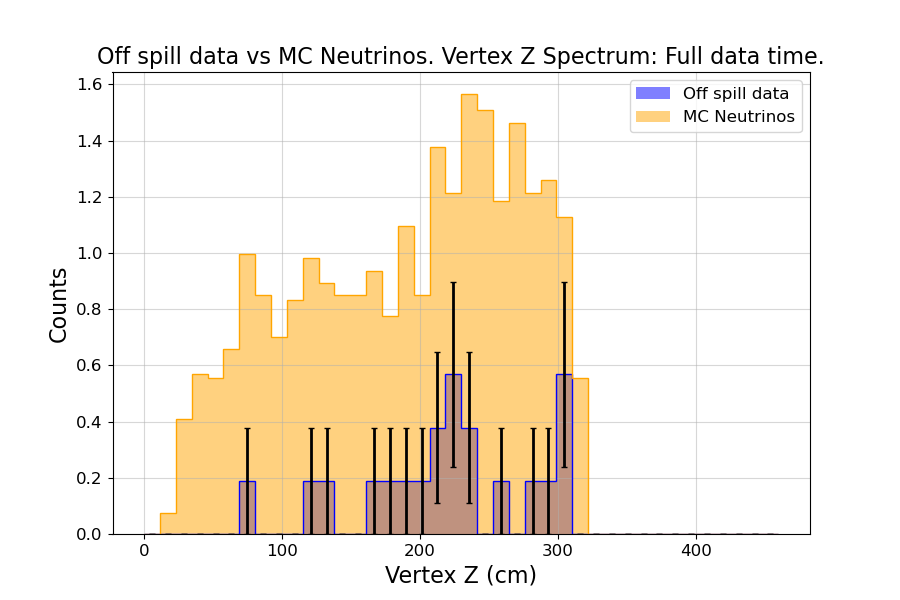
\includegraphics[width=0.32\linewidth]{sections/appendix/w133_yescut_fulltime/sig_bkg_vertexZ_spectrum_full_sig_time.png}
    \caption{Left: Vertex position in Z before cuts, area normalized to 1. Middle: Vertex position in Z with all other cuts applied, area normalized to 1. Right: Vertex position in Z with all other cuts applied, normalized to the expected number of events in the available data.}
    \label{fig:vertexZ}
\end{figure}

\begin{figure}[!h]
    \centering
    
\includegraphics[width=0.32\linewidth]{sections/appendix/w133_nocut_normalized/sig_bkg_vertexY_spectrum_normalized.png}
    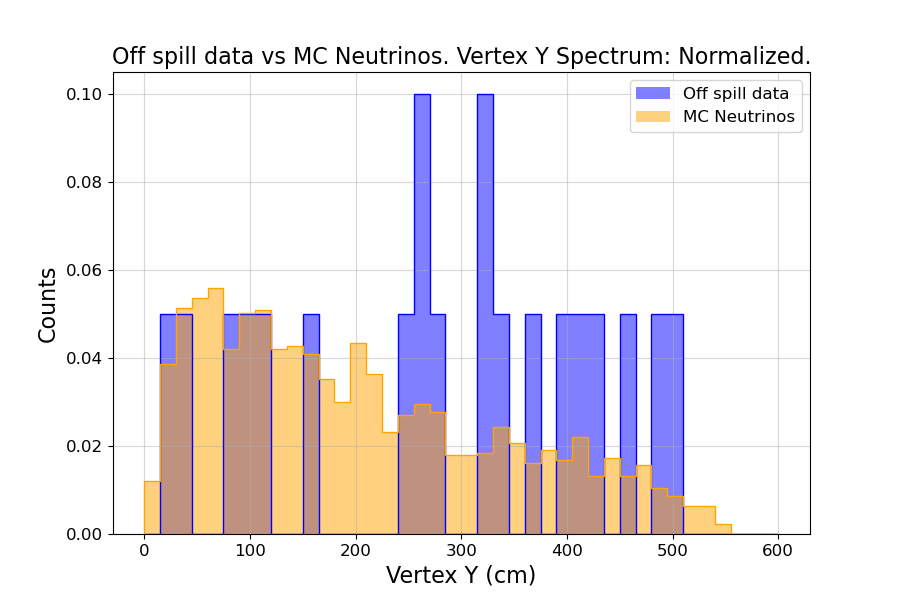
\includegraphics[width=0.32\linewidth]{sections/appendix/w133_yescut_normalized/sig_bkg_vertexY_spectrum_normalized.png}
    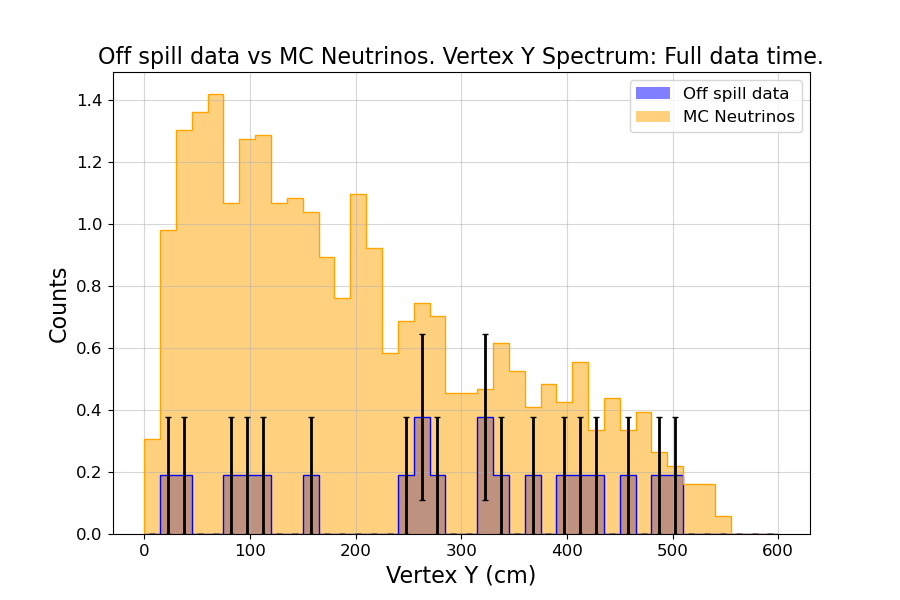
\includegraphics[width=0.32\linewidth]{sections/appendix/w133_yescut_fulltime/sig_bkg_vertexY_spectrum_full_sig_time.png}
    \caption{Left: Vertex position in Y before cuts, area normalized to 1. Middle: Vertex position in Y with all other cuts applied, area normalized to 1. Right: Vertex position in Y with all other cuts applied, normalized to the expected number of events in the available data.}
    \label{fig:vertexY}
\end{figure}


\begin{figure}[!h]
    \centering
    
\includegraphics[width=0.32\linewidth]{sections/appendix/w133_nocut_normalized/sig_bkg_ROI_Z_size_spectrum_normalized.png}
    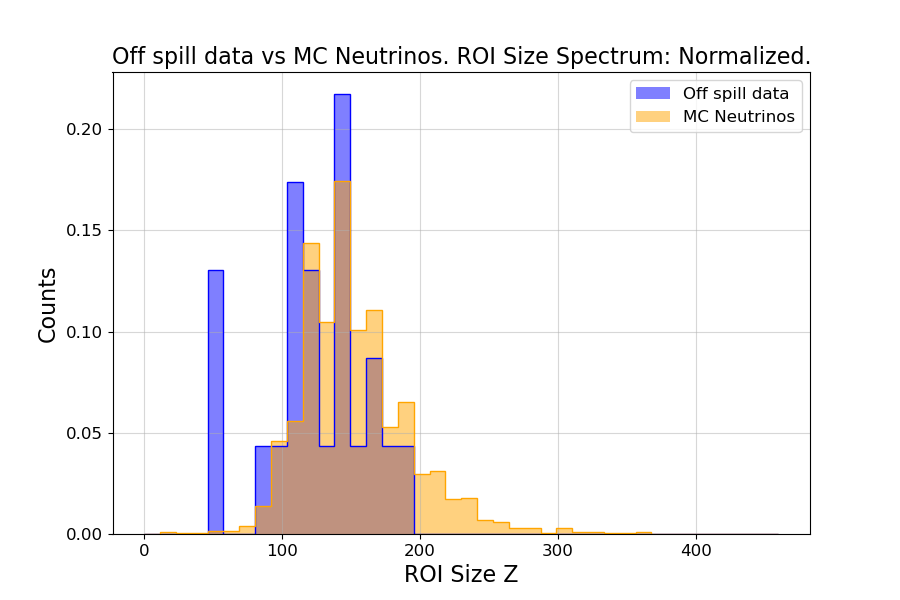
\includegraphics[width=0.32\linewidth]{sections/appendix/w133_yescut_normalized/sig_bkg_ROI_Z_size_spectrum_normalized.png}
    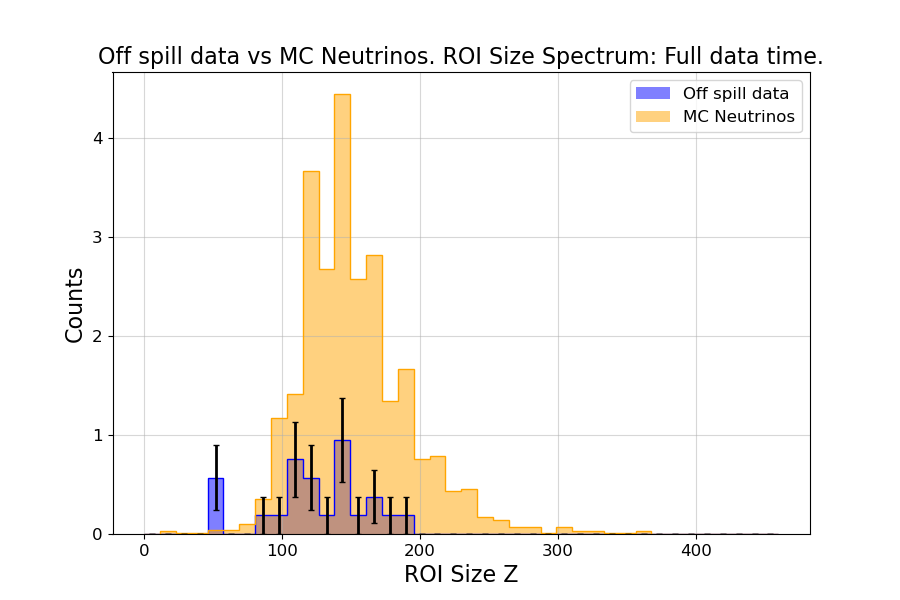
\includegraphics[width=0.32\linewidth]{sections/appendix/w133_yescut_fulltime/sig_bkg_ROI_Z_size_spectrum_full_sig_time.png}
    \caption{Left: ROI size distribution before cuts, area normalized to 1. Middle: ROI size distribution  with all other cuts applied, area normalized to 1. Right: ROI size distribution with all other cuts applied, normalized to the expected number of events in the available data.}
    \label{fig:ROIsize}
\end{figure}







 